% Copyright (c) 2015 Daniele Masini - d.masini.it@gmail.com

\chapter{Congruenza nei 
triangoli}\label{chap:congruenza_nei_triangoli}

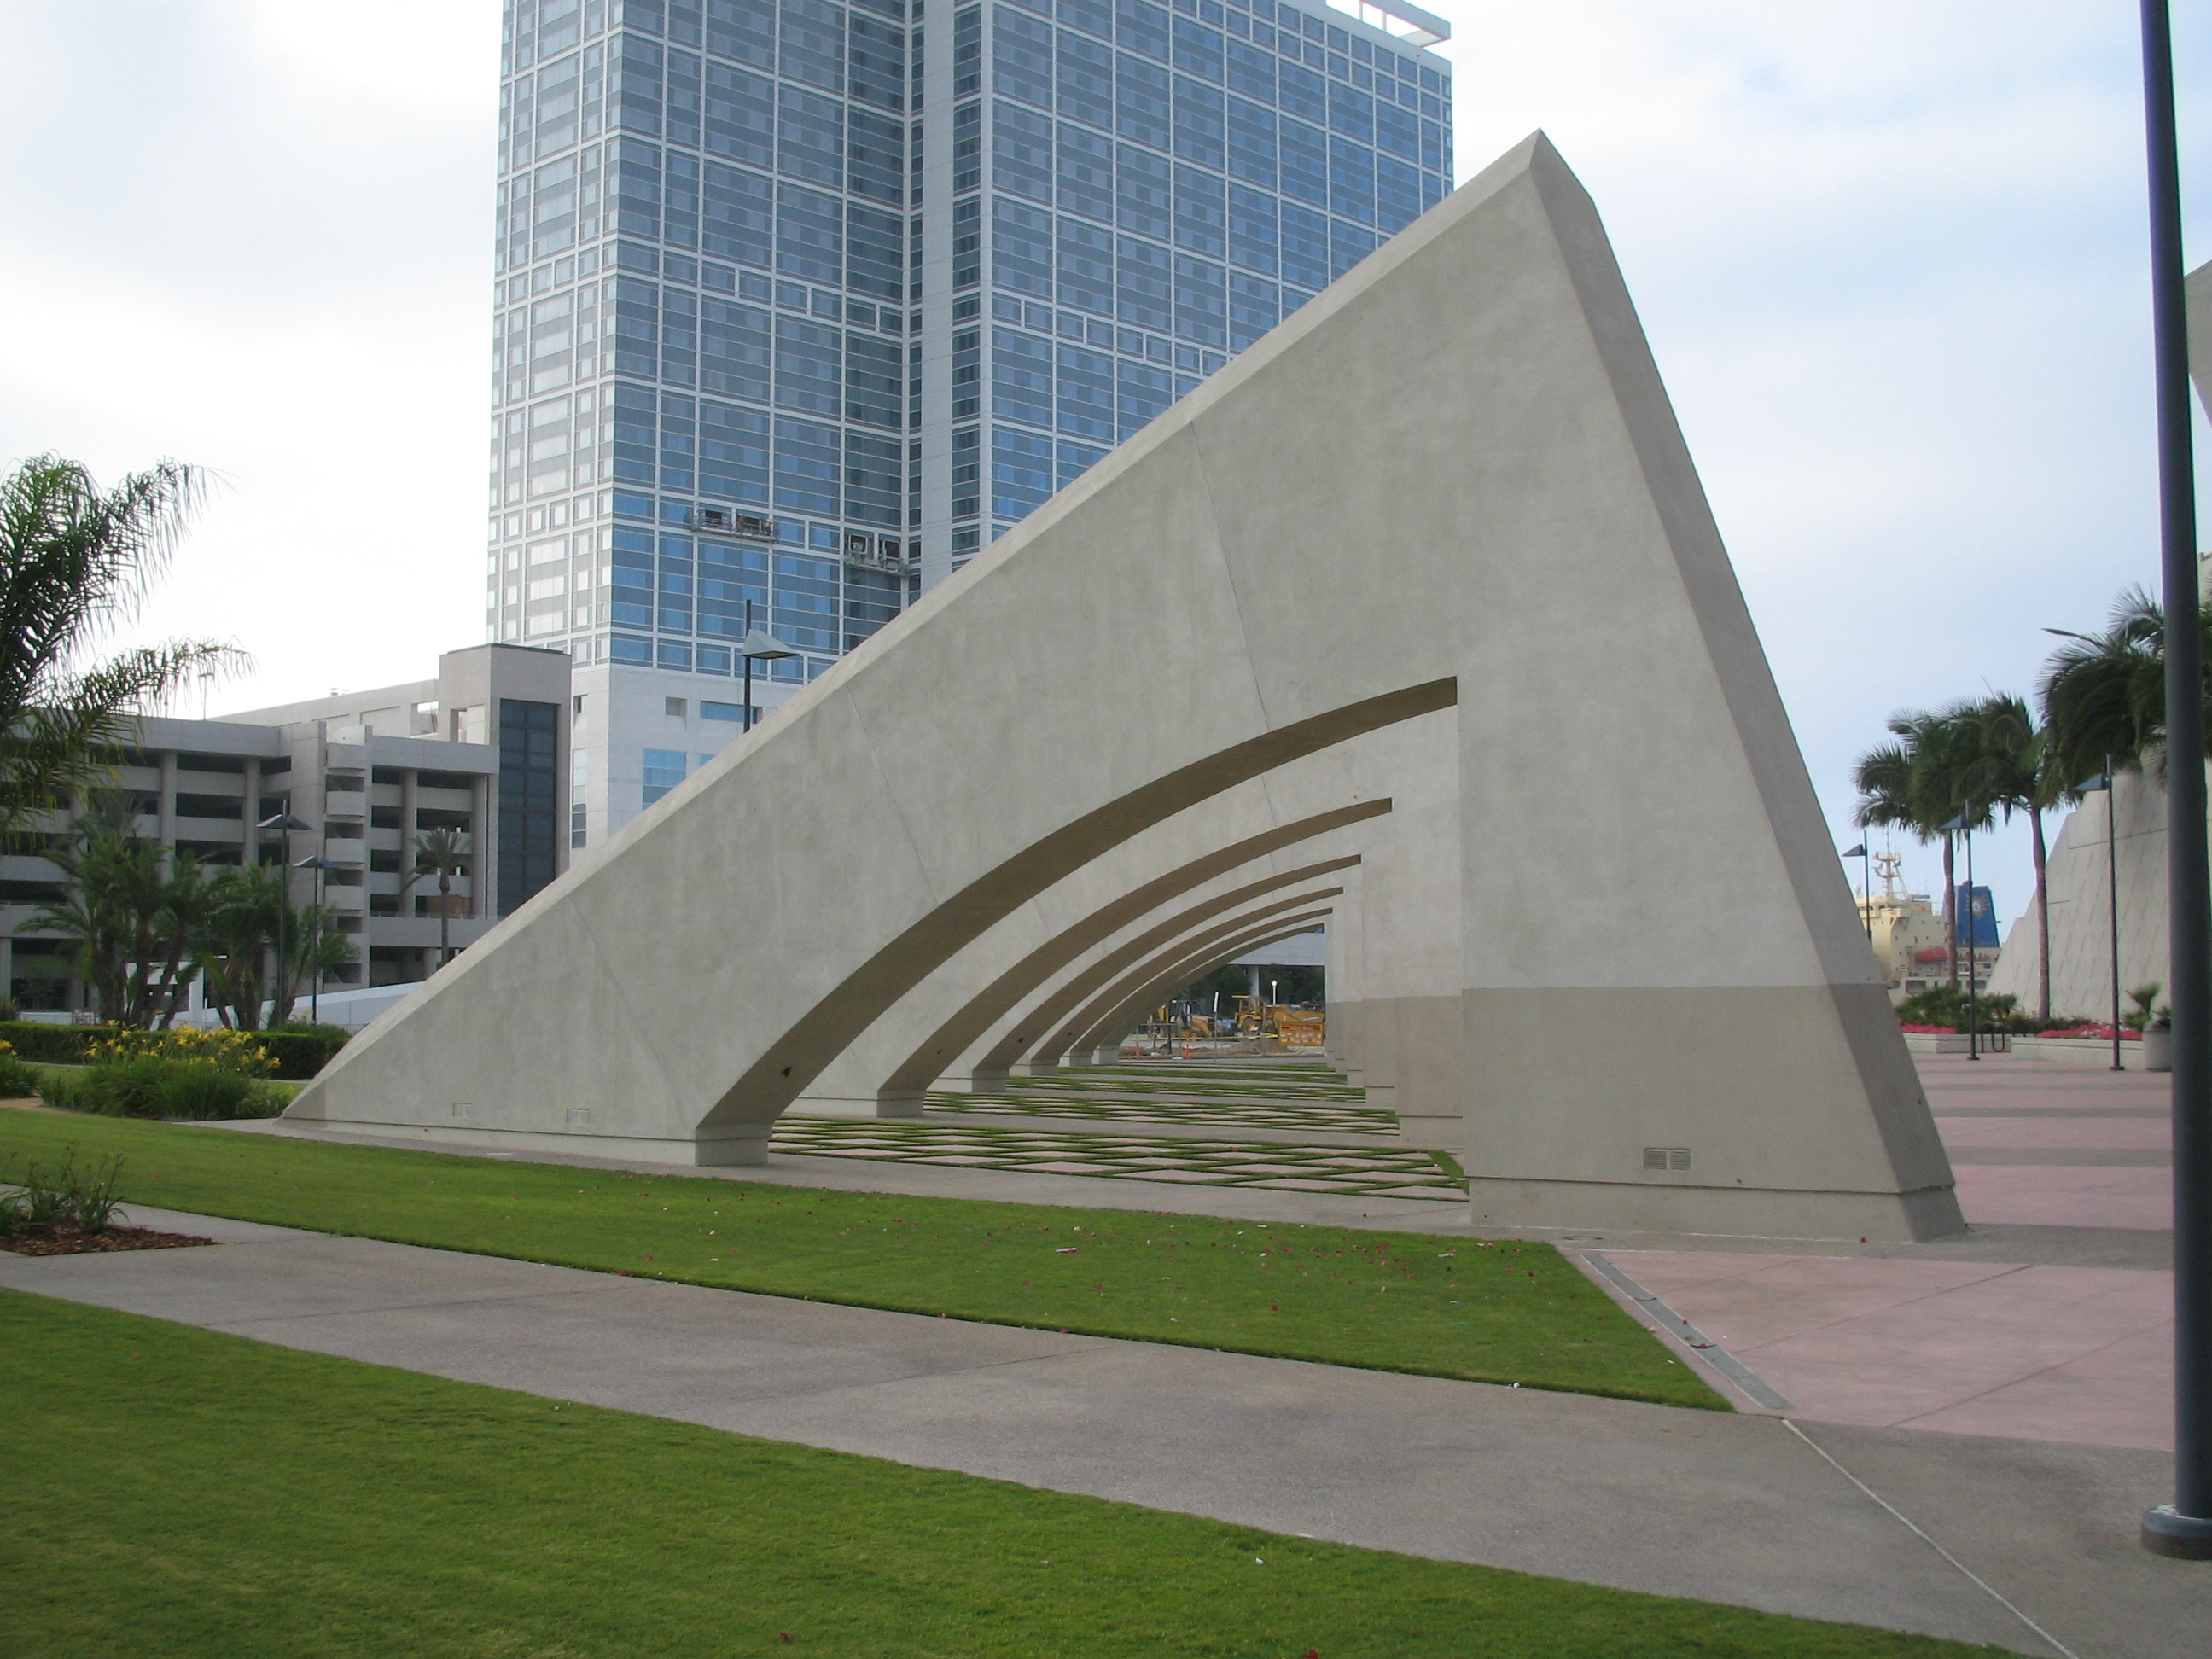
\includegraphics[width=0.95\textwidth]{\folder img/triangle_shapes.jpg}
  \begin{center}
    {\large ``Triangle Shapes''}\par
    Foto di maxtodorov\par
    \url{http://www.flickr.com/photos/maxtodorov/3066505212/}\par
    Licenza: Creative Commons Attribution\par
  \end{center}
\newpage

\section{Definizioni relative ai 
triangoli}\label{sect:definizioni_triangoli}

Definiamo gli elementi principali di un triangolo
\begin{definizione}~
\begin{itemize*}
\item Un \emph{triangolo} è un poligono di tre lati.
\item Si chiamano \emph{vertici} gli estremi dei lati.
\item Un vertice si dice \emph{opposto a un lato} se non appartiene a 
quel lato.
\item Si chiamano \emph{angoli interni} del triangolo i tre angoli 
formati dai lati.
\item Un angolo interno si dice \emph{angolo compreso tra due lati} 
quando i lati dell'angolo contengono dei lati del triangolo.
\item Un angolo interno si dice \emph{angolo adiacente a un lato} del 
triangolo quando uno dei suoi lati contiene quel lato del triangolo.
\item Un angolo si dice \emph{angolo esterno} al triangolo se è un 
angolo adiacente a un angolo interno.
\item Si dice \emph{bisettrice} relativa a un vertice, il segmento di 
bisettrice dell'angolo al vertice che ha per estremi il vertice 
stesso e il punto in cui essa incontra il lato opposto.
\item Si dice \emph{mediana} relativa a un lato il segmento che ha 
per estremi il punto medio del lato e il vertice opposto a quel lato.
\item Si dice \emph{altezza} di un triangolo relativa a un suo lato 
il segmento di perpendicolare che ha per estremi il vertice opposto 
al lato e il punto di intersezione della perpendicolare con la retta 
contenente il lato. 
\item Si dice \emph{asse} di un triangolo, relativo a un suo lato, la 
perpendicolare al lato condotta nel suo punto medio.
\end{itemize*}
\end{definizione}

Nel triangolo (a) della figura seguente, $A$, $B$ e $C$ sono i 
vertici del triangolo, il vertice $A$ è opposto al lato $a$, l'angolo 
$\alpha$ è interno al triangolo ed è compreso tra i lati $AB$ e $AC$, 
mentre l'angolo $\beta$ è esterno. Nel triangolo (b) $AL$ è la 
bisettrice dell'angolo nel vertice $A$, $AH$ è altezza relativa alla 
base $BC$, $AM$ è la mediana relativa al lato $BC$ e la retta $r$ è 
l'asse di $BC$.


\begin{inaccessibleblock}[Figura: TODO]
 \begin{figure}[htb]
\centering% Copyright (c) 2015 Daniele Masini - d.masini.it@gmail.com

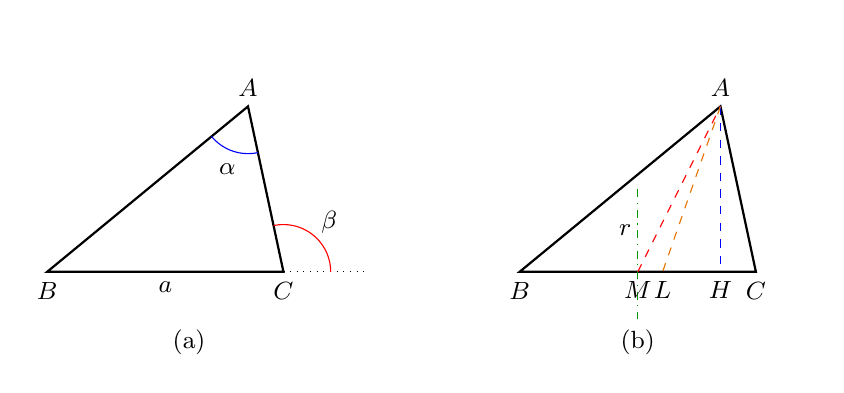
\begin{tikzpicture}[scale=1.5,font=\small]
\usetikzlibrary{calc}

\begin{scope}

\coordinate (b) at (0,0);
\coordinate (a) at (1.7,1.4);
\coordinate (c) at (2,0);

\draw[thick] (b) node[below] {$B$} -- node[below,midway] {$a$} (c) node[below] {$C$} -- (a) node[above] {$A$} -- cycle;
\draw[dotted] (c) -- ($(b)!1.35!(c)$) coordinate (d);

\begin{scope}
\clip (c) -- (d) -- (2.5,1) -- (a) -- cycle;
\draw[red] (c) circle (0.4);
\end{scope}
\node at ([shift={(11pt,12pt)}]c) {$\beta$};

\begin{scope}
\clip (b) -- (a) -- (c) -- cycle;
\draw[blue] (a) circle (0.4);
\end{scope}
\node at ([shift={(-5pt,-15pt)}]a) {$\alpha$};

\node at (1.2,-0.6) {(a)};

%\node at (2.5,1.2) {angolo};
%\node at (2.5,0.9) {esterno};
\end{scope}

\begin{scope}[xshift=4cm]

\coordinate (b) at (0,0);
\coordinate (a) at (1.7,1.4);
\coordinate (c) at (2,0);

\draw[thick] (b) node[below] {$B$} -- (c) node[below] {$C$} -- (a) node[above] {$A$} -- cycle;

%\begin{scope}
%\clip (b) -- (a) -- (c) -- cycle;
%\draw (a) node[left=3pt, below=15pt] {$\alpha$} circle (0.4);
%\end{scope}

\coordinate (m) at ($(b)!0.5!(c)$);

\draw[green!60!black,dashdotted] ($(m)!0.7cm!90:(c)$) coordinate (r) -- ($(m)!-.4cm!90:(c)$); % asse
\node at ([shift={(-3pt,-10pt)}]r) {$r$};
\draw[red,dashed] (m) node[black,below] {$M$} -- (a); % mediana
\draw[blue,dashed] (a) -- ($(b)!(a)!(c)$) node[black,below] {$H$}; % altezza

\node [circle] (circ1) at (a) [minimum size=2cm] {}; % circonferenza con centro in A
\coordinate (u) at (intersection of a--b and circ1);
\coordinate (v) at (intersection of a--c and circ1);
\node [circle] (circ2) at (u) [minimum size=2cm] {}; % circonferenza con centro in U
\node [circle] (circ3) at (v) [minimum size=2cm] {}; % circonferenza con centro in V
\coordinate (bis) at (intersection 1 of circ2 and circ3);
% la bisettrice di A passa per A e per bis1
\coordinate (bi) at ($(a)!5!(bis)$);
\coordinate (bt) at (intersection of b--c and a--bi);
\draw[orange!90!black,dashed] (a) -- (bt) node [black,below] {$L$}; % bisettrice


\node at (1,-0.6) {(b)};
\end{scope}

\end{tikzpicture}

\caption{Triangolo. Vertici, angoli, bisettrice, mediana, asse.}
\label{fig:triangolo1}
\end{figure}
\end{inaccessibleblock}

I triangoli possono essere classificati rispetto ai lati
\begin{definizione}~
\begin{itemize*}
\item un triangolo si dice \emph{equilatero} se ha i tre lati 
congruenti;
\item un triangolo si dice \emph{isoscele} se ha (almeno) due lati 
congruenti;
\item un triangolo si dice \emph{scaleno} se ha i lati a due a due 
non congruenti.
\end{itemize*}
\end{definizione}


\begin{inaccessibleblock}[Figura: TODO]
 \begin{figure}[htb]
\centering% Copyright (c) 2015 Daniele Masini - d.masini.it@gmail.com

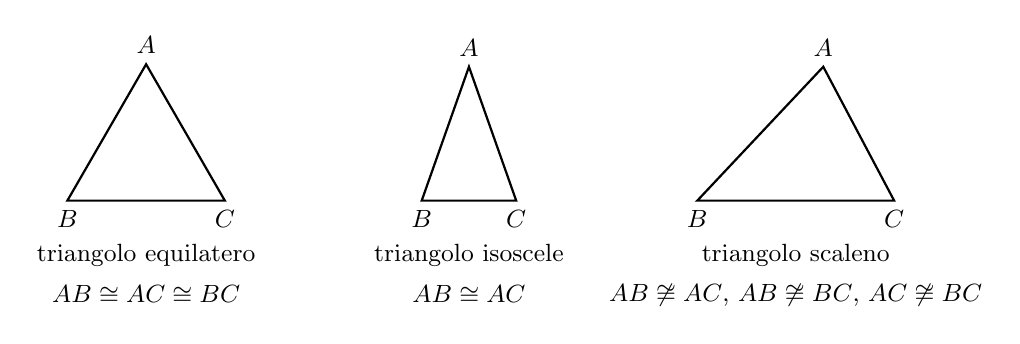
\begin{tikzpicture}[scale=1,font=\small]
\usetikzlibrary{calc}

\begin{scope}
\coordinate (b) at (0,0);
\coordinate (c) at (2,0);

\draw[thick] (b) node[below] {$B$} -- (c) node[below] {$C$} -- +(120:2) coordinate (a) node[above] {$A$} -- cycle;

\node at (1,-0.7) {triangolo equilatero};
\node at (1,-1.2) {$AB\cong AC\cong BC$};
\end{scope}

\begin{scope}[xshift=4.5cm]
\coordinate (b) at (0,0);
\coordinate (a) at (0.6,1.7);
\coordinate (c) at (1.2,0);

\draw[thick] (b) node[below] {$B$} -- (c) node[below] {$C$} -- (a) node[above] {$A$} -- cycle;

\node at (.6,-0.7) {triangolo isoscele};
\node at (.6,-1.2) {$AB\cong AC$};
\end{scope}


\begin{scope}[xshift=8cm]
\coordinate (b) at (0,0);
\coordinate (a) at (1.6,1.7);
\coordinate (c) at (2.5,0);

\draw[thick] (b) node[below] {$B$} -- (c) node[below] {$C$} -- (a) node[above] {$A$} -- cycle;

\node at (1.25,-0.7) {triangolo scaleno};
\node at (1.25,-1.2) {$AB\not\cong AC$, $AB\not\cong BC$, $AC\not\cong BC$};
\end{scope}

\end{tikzpicture}

\caption{Classificazione di un triangolo rispetto ai 
lati}\label{fig:class_triangolo_lati}
\end{figure}
\end{inaccessibleblock}

\noindent o rispetto agli angoli
\begin{definizione}~
\begin{itemize*}
\item un triangolo si dice \emph{rettangolo} se ha un angolo interno 
retto; in un triangolo rettangolo si chiama \emph{ipotenusa} il lato 
che si oppone all'angolo retto e si chiamano \emph{cateti} i lati 
adiacenti all'angolo retto;
\item un triangolo si dice \emph{ottusangolo} se ha un angolo interno 
ottuso;
\item un triangolo si dice \emph{acutangolo} se ha tutti gli angoli 
interni acuti.
\end{itemize*}
\end{definizione}


\begin{inaccessibleblock}[Figura: TODO]
 \begin{figure}[htb]
\centering% Copyright (c) 2015 Daniele Masini - d.masini.it@gmail.com

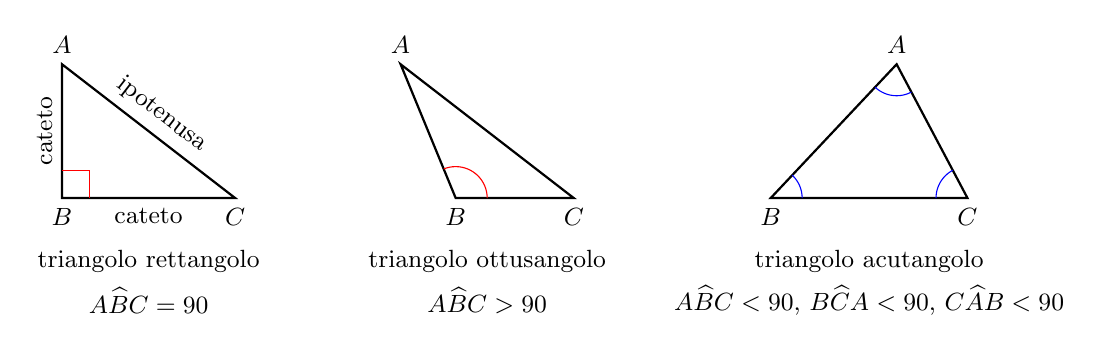
\begin{tikzpicture}[scale=1,font=\small]
\usetikzlibrary{calc}

\begin{scope}
\coordinate (a) at (0,1.7);
\coordinate (b) at (0,0);
\coordinate (c) at (2.2,0);

\draw[thick] (b) node[below] {$B$} -- node[below,midway,sloped] {cateto} (c) node[below] {$C$} -- node[above,midway,sloped] {ipotenusa} (a) node[above] {$A$} -- cycle;
\path (b) -- node[above,midway,sloped] {cateto} (a);
\draw[red] ([shift={(10pt,0)}]b) -- ([shift={(10pt,10pt)}]b) -- ([shift={(0pt,10pt)}]b);

\node at (1.1,-0.8) {triangolo rettangolo};
\node at (1.1,-1.3) {$A\widehat{B}C=90\grado$};
\end{scope}

\begin{scope}[xshift=5cm]
\coordinate (b) at (0,0);
\coordinate (a) at (-0.7,1.7);
\coordinate (c) at (1.5,0);

\draw[thick] (b) node[below] {$B$} -- (c) node[below] {$C$} -- (a) node[above] {$A$} -- cycle;

\begin{scope}
\clip (a) -- (b) -- (c) -- (1.5,1.7) -- cycle;
\draw[red] (b) circle (0.4);
\end{scope}

\node at (.4,-0.8) {triangolo ottusangolo};
\node at (.4,-1.3) {$A\widehat{B}C>90\grado$};
\end{scope}

\begin{scope}[xshift=9cm]
\coordinate (b) at (0,0);
\coordinate (a) at (1.6,1.7);
\coordinate (c) at (2.5,0);

\draw[thick] (b) node[below] {$B$} -- (c) node[below] {$C$} -- (a) node[above] {$A$} -- cycle;

\begin{scope}
\clip (a) -- (b) -- (c) -- cycle;
\draw[blue] (b) circle (0.4);
\draw[blue] (a) circle (0.4);
\draw[blue] (c) circle (0.4);
\end{scope}

\node at (1.25,-0.8) {triangolo acutangolo};
\node at (1.25,-1.3) {$A\widehat{B}C<90\grado$, $B\widehat{C}A<90\grado$, $C\widehat{A}B<90\grado$};
\end{scope}

\end{tikzpicture}

\caption{Classificazione di un triangolo rispetto agli 
angoli}\label{fig:class_triangolo_angoli}
\end{figure}
\end{inaccessibleblock}

\section{Primo e secondo criterio di congruenza dei 
triangoli}\label{sect:primo_secondo_criterio_di_congruenza_triangoli}

Ricordiamo che due figure piane si dicono \emph{congruenti} se sono 
sovrapponibili, cioè se è possibile spostare una sull'altra, senza 
deformarle, in modo che coincidano perfettamente. 

In particolare, due triangoli sono sovrapponibili se hanno 
``ordinatamente'' congruenti i tre lati e i tre angoli. Con il 
termine ordinatamente intendiamo che, a partire da una coppia di 
vertici (il primo di un triangolo ed il secondo dell'altro) procedendo 
lungo il contorno in senso orario, oppure antiorario, incontriamo lati 
tra loro congruenti e vertici di angoli tra loro congruenti. Nel caso 
dei triangoli, questo succede esattamente quando angoli congruenti nei 
due triangoli sono compresi tra coppie di lati congruenti o, in 
maniera equivalente, quando sono opposti a lati congruenti.

I criteri di congruenza dei triangoli ci dicono che è sufficiente 
conoscere la congruenza di solo alcuni elementi dei due triangoli, 
generalmente tre elementi di un triangolo congruenti a tre elementi 
dell'altro triangolo, per poter affermare che i due triangoli sono 
tra loro congruenti, e quindi dedurne la congruenza degli altri 
elementi.

Un modo tradizionale di presentare l'argomento, dovuto allo stesso 
Euclide, è quello di ``dimostrare'' i primi due criteri di congruenza 
dei triangoli facendo uso della definizione stessa di congruenza come 
``uguaglianza per sovrapposizione'', e di utilizzarli successivamente 
per la verifica di altre proprietà.

Secondo il matematico tedesco Hilbert, il primo criterio di 
congruenza è invece un assioma e il secondo criterio può essere 
dimostrato per assurdo attraverso il primo. 

Presenteremo questi argomenti basilari alla maniera di Euclide.

\begin{teorema}[1\textsuperscript{o} Criterio di congruenza dei 
triangoli]
Due triangoli sono congruenti se hanno congruenti due lati e l'angolo 
tra essi compreso.
\end{teorema}

% figura ()

\begin{inaccessibleblock}[Figura: TODO]
 \begin{figure}[htb]
\centering% Copyright (c) 2015 Daniele Masini - d.masini.it@gmail.com

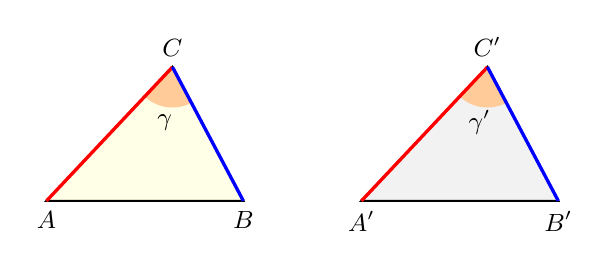
\begin{tikzpicture}[scale=1,font=\small]
\usetikzlibrary{calc}

\begin{scope}
\coordinate (a) at (0,0);
\coordinate (c) at (1.6,1.7);
\coordinate (b) at (2.5,0);
\draw[fill=yellow!10] (a) -- (b) -- (c) -- cycle;

\begin{scope}
\clip (a) -- (b) -- (c) -- cycle;
\draw[thick,orange!40,fill] (c) circle (0.5);
\node at ([shift={(-0.1,-0.7)}]c) {$\gamma$};
\end{scope}

\draw[thick] (a) node[below] {$A$} -- (b) node[below] {$B$} -- (c) node[above] {$C$} -- cycle;
\draw[red,very thick] (a) -- (c);
\draw[blue,very thick] (b) -- (c);

\end{scope}

\begin{scope}[xshift=4cm]
\coordinate (a) at (0,0);
\coordinate (c) at (1.6,1.7);
\coordinate (b) at (2.5,0);
\draw[fill=gray!10] (a) -- (b) -- (c) -- cycle;

\begin{scope}
\clip (a) -- (b) -- (c) -- cycle;
\draw[thick,orange!40,fill] (c) circle (0.5);\node at ([shift={(-0.1,-0.7)}]c) {$\gamma'$};
\end{scope}

\draw[thick] (a) node[below] {$A'$} -- (b) node[below] {$B'$} -- (c) node[above] {$C'$} -- cycle;
\draw[red,very thick] (a) -- (c);
\draw[blue,very thick] (b) -- (c);

\end{scope}

\end{tikzpicture}

\end{figure}
\end{inaccessibleblock}

\noindent Ipotesi: $AC\cong A'C'$, $BC\cong B'C'$, $\gamma \cong 
\gamma'$.\tab Tesi:  $ABC \cong A'B'C'$.

\begin{proof}
Vogliamo dimostrare che il triangolo $A’B’C’$ può essere portato a 
sovrapporsi perfettamente al triangolo $ABC$.
A tal proposito, portiamo il punto $C’$ sul punto $C$ in modo tale 
che la semiretta $C’A’$ sia sovrapposta alla semiretta $CA$ ed i punti 
$B$ e $B’$ siano nello stesso semipiano individuato dalla retta $AC$.
% Dopo questo movimento, i triangoli potrebbero trovarsi nella 
% posizione della figura a lato?
Poiché per ipotesi i segmenti $AC$ e $A’C’$ sono congruenti, se $C$ 
coincide con $C’$ anche $A$ deve coincidere con $A’$.
%, mentre nella figura $A’C’$ è maggiore di $AC$. Né $A'$ può cadere 
% all'interno di $AC$. In definitiva $C\equiv C'$ e $A\equiv A'$.

% Allora i triangoli potrebbero trovarsi almeno nella seguente 
% posizione, nella quale $A$ e $A’$ coincidono?
% Tuttavia nemmeno questa posizione è possibile poiché
Avendo supposto per ipotesi che gli angoli $\gamma$ e $\gamma'$ sono 
congruenti, la semiretta per $CB$ e la semiretta per $C’B’$ devono 
sovrapporsi, in quanto devono formare lo stesso angolo con la 
semiretta per $CA$, ovvero per $C'A'$.

A questo punto, rimane da fissare la posizione di $B’$ rispetto a 
$B$, cioè rimane da decidere se $B’$ cade internamente al segmento 
$CB$, come nella figura che segue, se $B’$ cade esternamente al 
segmento $CB$ o se $B’$ e $B$ coincidono.
Inoltre, poiché per ipotesi $BC\cong B'C'$, il punto $B’$ deve 
necessariamente coincidere con $B$.

Pertanto tutti i vertici del triangolo $A'B'C'$ si sovrappongono ai 
vertici del triangolo $ABC$ e di conseguenza i triangoli $ABC$ e 
$A’B’C’$ sono congruenti.
\end{proof}

\begin{teorema}[2\textsuperscript{o} Criterio di congruenza dei 
triangoli]
Due triangoli sono congruenti se hanno congruenti due angoli e il 
lato tra essi compreso.
\end{teorema}


\begin{inaccessibleblock}[Figura: TODO]
 \begin{figure}[htb]
\centering% Copyright (c) 2015 Daniele Masini - d.masini.it@gmail.com

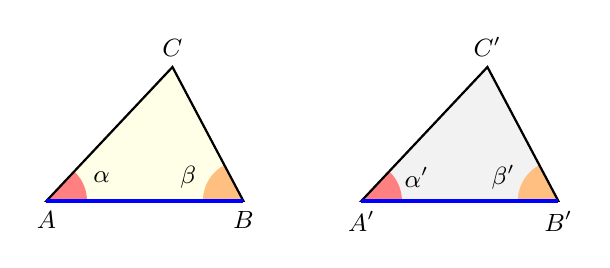
\begin{tikzpicture}[scale=1,font=\small]
\usetikzlibrary{calc}

\begin{scope}
\coordinate (a) at (0,0);
\coordinate (c) at (1.6,1.7);
\coordinate (b) at (2.5,0);
\draw[fill=yellow!10] (a) -- (b) -- (c) -- cycle;

\begin{scope}
\clip (a) -- (b) -- (c) -- cycle;
\draw[thick,red!50,fill] (a) circle (0.5);
\node at ([shift={(0.7,0.3)}]a) {$\alpha$};
\draw[thick,orange!50,fill] (b) circle (0.5);
\node at ([shift={(-0.7,0.3)}]b) {$\beta$};
\end{scope}

\draw[thick] (a) node[below] {$A$} -- (b) node[below] {$B$} -- (c) node[above] {$C$} -- cycle;
\draw[blue,very thick] (a) -- (b);


\end{scope}

\begin{scope}[xshift=4cm]
\coordinate (a) at (0,0);
\coordinate (c) at (1.6,1.7);
\coordinate (b) at (2.5,0);
\draw[fill=gray!10] (a) -- (b) -- (c) -- cycle;

\begin{scope}
\clip (a) -- (b) -- (c) -- cycle;
\draw[thick,red!50,fill] (a) circle (0.5);
\node at ([shift={(0.7,0.3)}]a) {$\alpha'$};
\draw[thick,orange!50,fill] (b) circle (0.5);
\node at ([shift={(-0.7,0.3)}]b) {$\beta'$};
\end{scope}

\draw[thick] (a) node[below] {$A'$} -- (b) node[below] {$B'$} -- (c) node[above] {$C'$} -- cycle;
\draw[blue,very thick] (a) -- (b);

\end{scope}

\end{tikzpicture}

\end{figure}
\end{inaccessibleblock}

\noindent Ipotesi: $AB\cong A'B'$, $\alpha\cong \alpha'$, $\beta 
\cong \beta'$.\tab Tesi:  $ABC \cong A'B'C'$.

\begin{proof}
Vogliamo dimostrare che il triangolo $A'B'C'$ può essere portato a 
sovrapporsi perfettamente al triangolo $ABC$.
A tal proposito, in virtù della congruenza dei lati $AB$ e $A'B'$, 
portiamo a sovrapporre il segmento $A'B'$ al segmento $AB$ in maniera 
tale che $A'$ coincida con $A$, $B'$ coincida con $B$ e i punti $C$ e 
$C'$ siano nello stesso semipiano individuato dalla retta $AB$. 

% I due triangoli potrebbero trovarsi nella posizione rappresentata a 
% fianco?
Dalla congruenza degli angoli $\alpha$ e $\alpha'$ segue che la 
semiretta $A'C'$ sarà sovrapposta alla semiretta $AC$; analogamente, 
dalla congruenza degli angoli $\beta$ e $\beta'$ segue che la 
semiretta $B'C'$ sarà sovrapposta alla semiretta $BC$. Dunque $C$ e 
$C'$ devono necessariamente coincidere, perché sono l'unica 
intersezione di due rette incidenti.

Poiché, dunque, i tre vertici si sono sovrapposti, i due triangoli 
sono completamente sovrapposti e quindi sono congruenti.
\end{proof}

\begin{exrig}
\begin{esempio}\label{esempio:2.1}
Si considerino due rette incidenti, $r$ ed $s$, ed il loro punto in 
comune $P$. Sulle semirette opposte di origine $P$ si prendano punti 
equidistanti da $P$, come in figura, in maniera tale che $AP\cong 
PB$, $CP\cong PD$. Dimostra che, unendo i quattro punti in modo da 
costruire un quadrilatero, i quattro triangoli che si vengono a 
formare sono a due a due congruenti: $ACP\cong BDP$, $ADP\cong BPC$.

Realizziamo il disegno (figura~\ref{fig:esempio2.1}) ed esplicitiamo 
ipotesi e tesi.


\begin{inaccessibleblock}[Figura: TODO]
 \begin{figure}[htb]
\centering% Copyright (c) 2015 Daniele Masini - d.masini.it@gmail.com

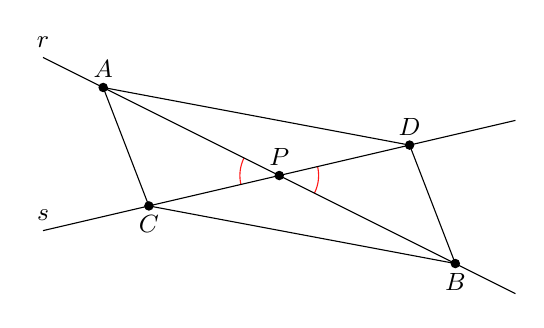
\begin{tikzpicture}[scale=1,font=\small]
\usetikzlibrary{calc}

\begin{scope}
\coordinate (s1) at (-3,-0.7);
\coordinate (s2) at (3,0.7);
\coordinate (r1) at (-3,1.5);
\coordinate (r2) at (3,-1.5);

\coordinate (p) at (intersection of r1--r2 and s1--s2);
\coordinate (a) at ($(p)!2.5cm!(r1)$);
\coordinate (b) at ($(p)!2.5cm!(r2)$);
\coordinate (c) at ($(p)!1.7cm!(s1)$);
\coordinate (d) at ($(p)!1.7cm!(s2)$);
\draw[fill] (a) circle (1.5pt) node[above] {$A$};
\draw[fill] (b) circle (1.5pt) node[below] {$B$};
\draw[fill] (c) circle (1.5pt) node[below] {$C$};
\draw[fill] (d) circle (1.5pt) node[above] {$D$};
\draw (a) -- (c) -- (b) -- (d) -- cycle;

\begin{scope}
\clip (a) -- (p) -- (c) -- cycle;
\draw[red!90] (p) circle (0.5);
%\node at ([shift={(0.7,0.3)}]p) {$\alpha$};
\end{scope}

\begin{scope}
\clip (b) -- (p) -- (d) -- cycle;
\draw[red!90] (p) circle (0.5);
%\node at ([shift={(0.7,0.3)}]p) {$\alpha$};
\end{scope}
\draw (s1) node[above] {$s$} -- (s2);
\draw (r1) node[above] {$r$} -- (r2);
\draw[fill] (p) circle (1.5pt) node[above] {$P$};

\end{scope}


\end{tikzpicture}

\caption{Esempio~\ref{esempio:2.1}}\label{fig:esempio2.1}
\end{figure}
\end{inaccessibleblock}

\noindent Ipotesi: $r\cap s=P$, $AP\cong PB$, $CP\cong PD$.\tab\tab 
Tesi: $ACP\cong BDP$, $ADP\cong BPC$.

\begin{proof}
I triangoli $ACP$ e $BPD$ hanno: $AP\cong PB$ per ipotesi, $CP\cong 
PD$ per ipotesi, $A\widehat{P}C\cong B\widehat{P}D$ perché opposti al 
vertice. Pertanto sono congruenti per il 1\textsuperscript{o} 
criterio di congruenza dei triangoli.

Analogamente, i triangoli $ADP$ e $BPC$ hanno: 
\ldots\ldots\ldots\ldots\ldots\ldots\ldots
\end{proof}
\end{esempio}

\begin{esempio}\label{esempio:2.2}
Si considerino un segmento $AB$ ed il suo punto medio $M$. Si tracci 
una generica retta $r$ passante per $M$ e distinta dalla retta per 
$AB$. Si traccino inoltre due semirette di origine rispettivamente 
$A$ e $B$, situate nei due semipiani opposti rispetto alla retta per 
$AB$, che intersechino la retta $r$ rispettivamente in $C$ e in $D$ e 
che formino con la retta per $AB$ due angoli congruenti (vedi 
figura~\ref{fig:esempio2.2}). Detti $C$ e $D$ i rispettivi punti di 
intersezione delle due semirette con la retta $r$, dimostra che i 
triangoli $AMC$ e $BMD$ sono congruenti.


\begin{inaccessibleblock}[Figura: TODO]
 \begin{figure}[htb]
\centering% Copyright (c) 2015 Daniele Masini - d.masini.it@gmail.com

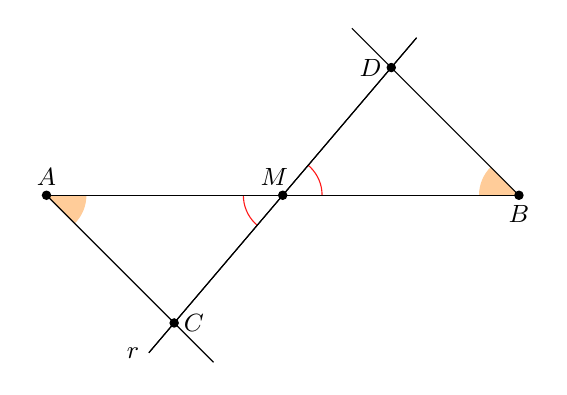
\begin{tikzpicture}[scale=1,font=\small]
\usetikzlibrary{calc}

\begin{scope}
\coordinate (a) at (-3,0);
\coordinate (b) at (3,0);
\coordinate (m) at (0,0);
\coordinate (r1) at (-1.7,-2);
\coordinate (r2) at (1.7,2);
\coordinate (s1) at ([shift={(135:3)}]b);
\coordinate (t1) at ([shift={(-45:3)}]a);
\coordinate (c) at (intersection of r1--r2 and a--t1);
\coordinate (d) at (intersection of r1--r2 and b--s1);

\begin{scope}
\clip (a) -- (m) -- (c) -- cycle;
\draw[fill,orange!40] (a) circle (0.5);
\draw[red!90] (m) circle (0.5);
%\node at ([shift={(0.7,0.3)}]p) {$\alpha$};
\end{scope}

\begin{scope}
\clip (b) -- (m) -- (d) -- cycle;
\draw[fill,orange!40] (b) circle (0.5);
\draw[red!90] (m) circle (0.5);
%\node at ([shift={(0.7,0.3)}]p) {$\alpha$};
\end{scope}

\draw[fill] (a) circle (1.5pt) node[above] {$A$};
\draw[fill] (b) circle (1.5pt) node[below] {$B$};
\draw[fill] (c) circle (1.5pt) node[right] {$C$};
\draw[fill] (d) circle (1.5pt) node[left] {$D$};
\draw (a) -- (b);
\draw (r1) -- (r2);
\draw (a) -- (t1);
\draw (b) -- (s1);

\draw (r1) node[left] {$r$} -- (r2);
\draw[fill] (m) circle (1.5pt) node[left = 3pt, above=0pt] {$M$};

\end{scope}


\end{tikzpicture}

\caption{Esempio~\ref{esempio:2.2}}\label{fig:esempio2.2}
\end{figure}
\end{inaccessibleblock}

\noindent Ipotesi: $AM\cong MB$, $M\widehat{A}C\cong 
M\widehat{B}D$.\tab Tesi: $AMC\cong BMD$.

\begin{proof}
I segmenti $AM$ e $MB$ sono congruenti in quanto $M$ è il punto medio 
di $AB$, gli angoli di vertice $M$ sono congruenti perché opposti al 
vertice, gli angoli di vertici $A$ e $B$ sono congruenti per 
costruzione. Allora i triangoli $AMC$ e $BMD$ sono congruenti per il 
2\textsuperscript{o} criterio di congruenza dei triangoli.
\end{proof}
\end{esempio}
\end{exrig}

\section{Teoremi del triangolo 
isoscele}\label{sect:teoremi_triangolo_isoscele}

Il \emph{triangolo isoscele} ha almeno due lati congruenti, 
l'eventuale lato non congruente si chiama \emph{base}, i due lati 
congruenti si dicono \emph{lati obliqui}.

Il \emph{triangolo equilatero} è un caso particolare di triangolo 
isoscele: si dice che \emph{il triangolo equilatero è isoscele 
rispetto a qualsiasi lato preso come base}.

\begin{teorema}[del triangolo isoscele {[}teorema diretto{]}]
In un triangolo isoscele gli angoli alla base sono congruenti.
\end{teorema}


\begin{inaccessibleblock}[Figura: TODO]
 \begin{figure}[htb]
\centering% Copyright (c) 2015 Daniele Masini - d.masini.it@gmail.com

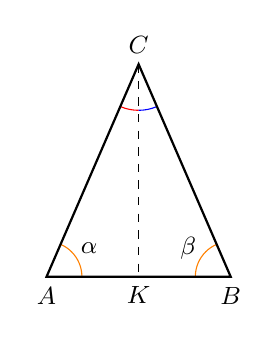
\begin{tikzpicture}[scale=0.9,font=\small]
\usetikzlibrary{calc}

\begin{scope}
\coordinate (a) at (-1.3,0);
\coordinate (b) at (1.3,0);
\coordinate (c) at (0,3);
\coordinate (k) at (0,0);

\begin{scope}
\clip (a) -- (b) -- (c) -- cycle;
\draw[orange] (a) circle (0.5);
\draw[orange] (b) circle (0.5);
\node at ([shift={(0.6,0.4)}]a) {$\alpha$};
\node at ([shift={(-0.6,0.4)}]b) {$\beta$};
\end{scope}

\begin{scope}
\clip (a) -- (c) -- (k) -- cycle;
\draw[red] (c) circle (0.65);
\end{scope}

\begin{scope}
\clip (b) -- (c) -- (k) -- cycle;
\draw[blue] (c) circle (0.65);
\end{scope}


\draw[thick] (a) node[below] {$A$} -- (b) node[below] {$B$} -- (c) node[above] {$C$} -- cycle;
\draw[dashed] (c) -- (k);
\node[below] at (k) {$K$};

\end{scope}


\end{tikzpicture}

\end{figure}
\end{inaccessibleblock}

\noindent Ipotesi: $AC\cong BC$.\tab Tesi: $\alpha\cong \beta$.

\begin{proof}
Tracciamo la bisettrice $CK$ dell'angolo in $C$.
I triangoli $ACK$ e $BCK$ sono congruenti per il primo criterio, 
infatti hanno:
\begin{itemize*}
\item $AC\cong CB$ per ipotesi;
\item $CK$ lato in comune;
\item $A\widehat{C}K\cong B\widehat{C}K$ perché $CK$ è la bisettrice 
dell'angolo in $C$.
\end{itemize*}
Pertanto, essendo congruenti, i due triangoli hanno tutti gli 
elementi congruenti, in particolare l'angolo $\alpha$ (in $A$) è 
congruente all'angolo $\beta$ (in $B$).
\end{proof}

Il teorema precedente è invertibile, nel senso che è valido anche il 
teorema inverso, quello che si ottiene scambiando tra loro ipotesi e 
tesi.

\begin{teorema}[del triangolo isoscele {[}teorema inverso{]}]
Se un triangolo ha due angoli congruenti, allora è isoscele (rispetto 
al lato compreso tra gli angoli congruenti preso come base).
\end{teorema}


\begin{inaccessibleblock}[Figura: TODO]
 \begin{figure}[htb]
\centering% Copyright (c) 2015 Daniele Masini - d.masini.it@gmail.com

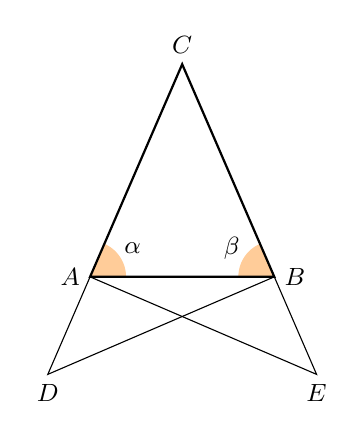
\begin{tikzpicture}[scale=0.9,font=\small]
\usetikzlibrary{calc}

\begin{scope}
\coordinate (a) at (-1.3,0);
\coordinate (b) at (1.3,0);
\coordinate (c) at (0,3);

\begin{scope}
\clip (a) -- (b) -- (c) -- cycle;
\draw[fill,orange!40] (a) circle (0.5);
\draw[fill,orange!40] (b) circle (0.5);
\node at ([shift={(0.6,0.4)}]a) {$\alpha$};
\node at ([shift={(-0.6,0.4)}]b) {$\beta$};
\end{scope}

\draw[thick] (a) node[left] {$A$} -- (b) node[right] {$B$} -- (c) node[above] {$C$} -- cycle;

\draw (a) -- ($(a)!-1.5cm!(c)$) node[below] {$D$} -- (b);
\draw (b) -- ($(b)!-1.5cm!(c)$) node[below] {$E$} -- (a);

\end{scope}


\end{tikzpicture}

\end{figure}
\end{inaccessibleblock}

\noindent Ipotesi: $\alpha\cong \beta$.\tab Tesi: $AC\cong BC$.

\begin{proof}
Procediamo per passi, realizzando una costruzione che ci permetta di 
confrontare coppie di triangoli congruenti. Prolunghiamo i lati $AC$ 
e $BC$ dalla parte di $A$ e di $B$ rispettivamente, e sui 
prolungamenti prendiamo due punti $D$ ed $E$ in maniera tale che 
risulti $AD\cong BE$.

Osserviamo che i triangoli $ADB$ e $BAE$ risultano congruenti per il 
1\textsuperscript{o} criterio, avendo in comune il lato $AB$ ed 
essendo $AD\cong BE$ per costruzione e $D\widehat{A}B\cong 
A\widehat{B}E$ perché adiacenti agli angoli $C\widehat{A}B$ e 
$C\widehat{B}A$ congruenti per ipotesi. Pertanto, tutti gli elementi 
dei due triangoli $ADB$ e $AEB$ sono ordinatamente congruenti, in 
particolare $DB\cong AE$, $A\widehat{D}B\cong B\widehat{E}A$ e 
$A\widehat{B}D\cong B\widehat{A}E$.

I triangoli $CDB$ e $CAE$ risultano dunque congruenti per il 
2\textsuperscript{o} criterio poiché hanno $DB\cong AE$, 
$C\widehat{D}B\cong C\widehat{E}A$ per quanto appena dimostrato e 
$C\widehat{D}B\cong C\widehat{A}E$ perché somma di angoli 
rispettivamente congruenti: $C\widehat{B}D\cong C\widehat{B}A + 
A\widehat{B}D$ e $C\widehat{A}E\cong C\widehat{A}B + B\widehat{A}E$.

Pertanto, i restanti elementi dei due triangoli risultano 
ordinatamente congruenti, in particolare $CB\cong CA$, che è la tesi 
che volevamo dimostrare.
\end{proof}


Dai due teoremi precedenti seguono importanti proprietà, che qui 
riportiamo come corollari.

\begin{corollario}
Un triangolo equilatero è anche equiangolo.
\end{corollario}

\begin{proof}
Poiché un triangolo equilatero è isoscele rispetto a qualsiasi lato 
preso come base, la tesi segue dal teorema diretto del triangolo 
isoscele.
\end{proof}

\begin{corollario}
Se un triangolo è equiangolo allora è equilatero.
\end{corollario}

\begin{proof}
Possiamo confrontare gli angoli a due a due; risulteranno i lati 
congruenti a due a due in base al teorema inverso del triangolo 
isoscele.
\end{proof}

\begin{corollario}
Un triangolo scaleno non ha angoli congruenti.
\end{corollario}

\begin{proof}
Se per assurdo un triangolo scaleno avesse due angoli congruenti, 
allora risulterebbe isoscele, in base al teorema inverso del 
triangolo isoscele.
\end{proof}

\begin{corollario}
Se un triangolo non ha angoli congruenti allora è scaleno.
\end{corollario}

\begin{proof}
Se un triangolo non ha angoli tra loro congruenti non può essere 
isoscele.
\end{proof}

\begin{proposizione}[Proprietà del triangolo isoscele]
In ogni triangolo isoscele, la mediana relativa alla base è anche 
altezza e bisettrice.
\end{proposizione}
Nella figura, $CJ$ è per ipotesi la bisettrice dell'angolo al vertice 
$\gamma_1$ del triangolo $ABC$, $FK$ è la mediana relativa alla base 
$DE$ del triangolo $DEF$, $IL$ è l'altezza relativa alla base $GH$ 
del triangolo $GHI$.


\begin{inaccessibleblock}[Figura: TODO]
 \begin{figure}[htb]
\centering% Copyright (c) 2015 Daniele Masini - d.masini.it@gmail.com

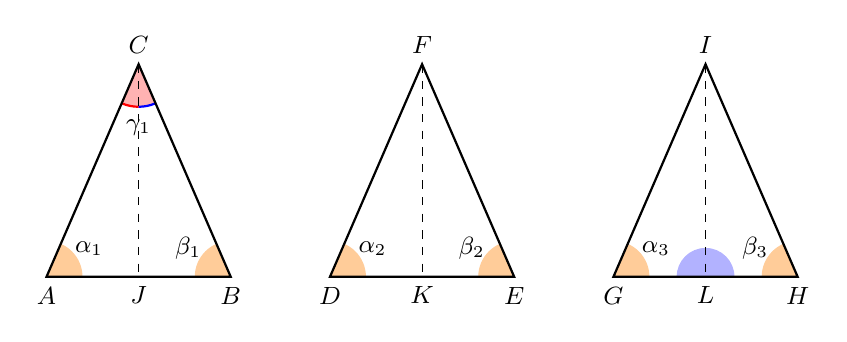
\begin{tikzpicture}[scale=0.9,font=\small]
\usetikzlibrary{calc}

\begin{scope}
\coordinate (a) at (-1.3,0);
\coordinate (b) at (1.3,0);
\coordinate (c) at (0,3);
\coordinate (j) at (0,0);

\begin{scope}
\clip (a) -- (b) -- (c) -- cycle;
\draw[fill,orange!40] (a) circle (0.5);
\draw[fill,orange!40] (b) circle (0.5);
\draw[fill,red!30] (c) circle (0.6);
\node at ([shift={(0.6,0.4)}]a) {$\alpha_1$};
\node at ([shift={(-0.6,0.4)}]b) {$\beta_1$};
\node at ([shift={(0,-0.9)}]c) {$\gamma_1$};
\end{scope}

\begin{scope}
\clip (a) -- (c) -- (j) -- cycle;
\draw[thick,red] (c) circle (0.6);
\end{scope}

\begin{scope}
\clip (b) -- (c) -- (j) -- cycle;
\draw[thick,blue] (c) circle (0.6);
\end{scope}

\draw[dashed] (c) -- (j) node[below] {$J$};
\draw[thick] (a) node[below] {$A$} -- (b) node[below] {$B$} -- (c) node[above] {$C$} -- cycle;

\end{scope}


\begin{scope}[xshift=4cm]
\coordinate (a) at (-1.3,0);
\coordinate (b) at (1.3,0);
\coordinate (c) at (0,3);
\coordinate (j) at (0,0);

\begin{scope}
\clip (a) -- (b) -- (c) -- cycle;
\draw[fill,orange!40] (a) circle (0.5);
\draw[fill,orange!40] (b) circle (0.5);
\node at ([shift={(0.6,0.4)}]a) {$\alpha_2$};
\node at ([shift={(-0.6,0.4)}]b) {$\beta_2$};
\end{scope}

\draw[dashed] (c) -- (j) node[below] {$K$};
\draw[thick] (a) node[below] {$D$} -- (b) node[below] {$E$} -- (c) node[above] {$F$} -- cycle;

\end{scope}

\begin{scope}[xshift=8cm]
\coordinate (a) at (-1.3,0);
\coordinate (b) at (1.3,0);
\coordinate (c) at (0,3);
\coordinate (j) at (0,0);

\begin{scope}
\clip (a) -- (b) -- (c) -- cycle;
\draw[fill,orange!40] (a) circle (0.5);
\draw[fill,orange!40] (b) circle (0.5);
\node at ([shift={(0.6,0.4)}]a) {$\alpha_3$};
\node at ([shift={(-0.6,0.4)}]b) {$\beta_3$};
\end{scope}

\begin{scope}
\clip (a) -- (b) -- (c) -- cycle;
\draw[fill,blue!30] (j) circle (0.4);
\end{scope}

\draw[dashed] (c) -- (j) node[below] {$L$};
\draw[thick] (a) node[below] {$G$} -- (b) node[below] {$H$} -- (c) node[above] {$I$} -- cycle;

\end{scope}

\end{tikzpicture}

\end{figure}
\end{inaccessibleblock}

Dividiamo l'enunciato in tre parti:
\begin{enumeratea}
\item In un triangolo isoscele la bisettrice dell'angolo al vertice è 
anche altezza e mediana relativa alla base.
\item In un triangolo isoscele la mediana relativa alla base è anche 
bisettrice dell'angolo al vertice e altezza relativa alla base.
\item In un triangolo isoscele l'altezza relativa alla base è anche 
bisettrice dell'angolo al vertice e mediana relativa alla base.
\end{enumeratea}

Per ciascuna di esse scriviamo ipotesi e tesi.
\begin{enumeratea}
\item In $ABC$:	Ipotesi: $AC\cong CB$, $\alpha_1\cong \beta_1$, 
$A\widehat{C}J\cong B\widehat{C}J$. Tesi: $CJ\perp AB$, $AJ\cong JB$.
\item In $DEF$:	\,Ipotesi: $DF\cong FE$, $\alpha_2\cong \beta_2$, 
$DK\cong KE$.\tab Tesi: $FK\perp DE$, $D\widehat{F}K\cong 
E\widehat{F}K$.
\item In $GHI$:	\,Ipotesi: $IG\cong IH$, $\alpha_3\cong \beta_3$, 
$IL\perp GH$.\tab Tesi: $GL\cong LH$, $G\widehat{I}L\cong 
H\widehat{I}L$.
\end{enumeratea}

\begin{proof}
Avviamo la dimostrazione delle prime due parti, che lasciamo 
completare al lettore e rimandiamo al prossimo capitolo la 
dimostrazione della terza.

\begin{enumeratea}
\item I triangoli $AJC$ e $CJB$ sono congruenti per il 
2\textsuperscript{o} criterio. Infatti hanno 
\ldots\ldots\ldots\ldots{}\\
Dunque $AJ\cong JB$ e $A\widehat{J}C\cong C\widehat{J}B$ che 
risultano pertanto retti in quanto adiacenti.  
\item I triangoli $DKF$ e $FKE$ sono congruenti per il 
1\textsuperscript{o} criterio. Infatti hanno 
\ldots\ldots\ldots\ldots{}\\
Dunque $D\widehat{F}K\cong E\widehat{F}K$ e $F\widehat{K}D\cong 
F\widehat{K}E$ che risultano pertanto retti in quanto adiacenti.
\end{enumeratea}
\end{proof}

\section{Terzo criterio di congruenza dei 
triangoli}\label{sect:terzo_criterio_congruenza_triangoli}

\begin{teorema}[3\textsuperscript{o} criterio di congruenza dei 
triangoli]
Due triangoli sono congruenti se hanno congruenti le tre coppie di 
lati.
\end{teorema}


\begin{inaccessibleblock}[Figura: TODO]
 \begin{figure}[htb]
\centering% Copyright (c) 2015 Daniele Masini - d.masini.it@gmail.com

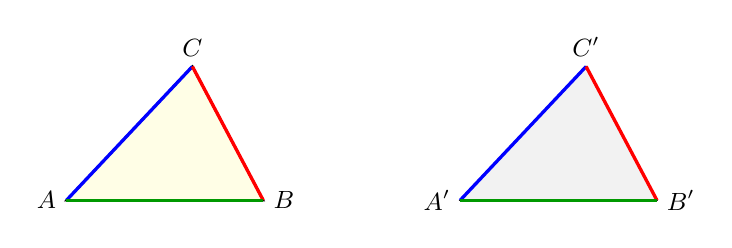
\begin{tikzpicture}[scale=1,font=\small]
\usetikzlibrary{calc}

\begin{scope}
\coordinate (a) at (0,0);
\coordinate (c) at (1.6,1.7);
\coordinate (b) at (2.5,0);

\draw[fill=yellow!10] (a) -- (b) -- (c) -- cycle;
\draw[thick] (a) node[left] {$A$} -- (b) node[right] {$B$} -- (c) node[above] {$C$} -- cycle;
\draw[blue,very thick] (a) -- (c);
\draw[red,very thick] (c) -- (b);
\draw[green!60!black,very thick] (a) -- (b);

\end{scope}

\begin{scope}[xshift=5cm]
\coordinate (a) at (0,0);
\coordinate (c) at (1.6,1.7);
\coordinate (b) at (2.5,0);

\draw[fill=gray!10] (a) node[left] {$A'$} -- (b) node[right] {$B'$} -- (c) node[above] {$C'$} -- cycle;
\draw[blue,very thick] (a) -- (c);
\draw[red,very thick] (c) -- (b);
\draw[green!60!black,very thick] (a) -- (b);

\end{scope}

\end{tikzpicture}

\end{figure}
\end{inaccessibleblock}

\noindent Ipotesi: $AB\cong A'B'$, $BC\cong B'C'$, $AC\cong 
A'C'$.\tab Tesi: $ABC\cong A'B'C'$.


\begin{inaccessibleblock}[Figura: TODO]
 \begin{figure}[htb]
\centering% Copyright (c) 2015 Daniele Masini - d.masini.it@gmail.com

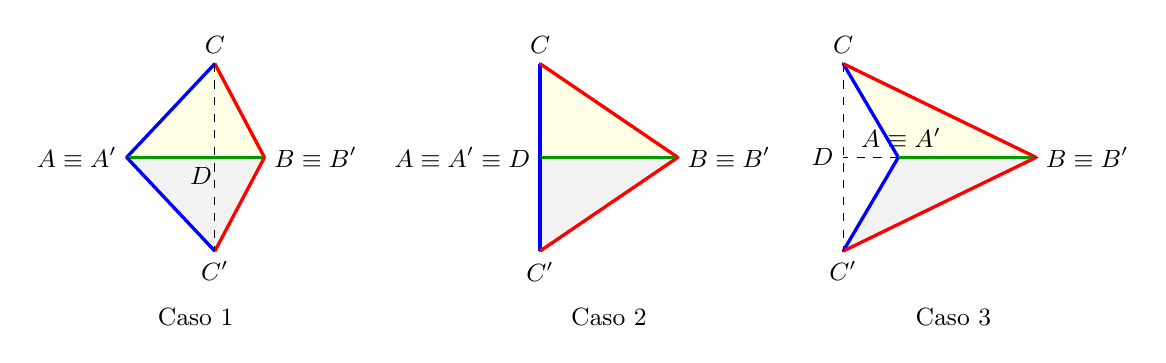
\begin{tikzpicture}[scale=.7,font=\small]
\usetikzlibrary{calc}

\begin{scope}
\coordinate (a) at (0,0);
\coordinate (c) at (1.6,1.7);
\coordinate (b) at (2.5,0);
\coordinate (c1) at (1.6,-1.7);

\draw[fill=gray!10] (a) -- (b) -- (c1) -- cycle;

\draw[fill=yellow!10] (a) -- (b) -- (c) -- cycle;
\draw (a) node[left] {$A\equiv A'$} -- (b) node[right] {$B\equiv B'$} -- (c) node[above] {$C$} -- cycle;
\draw[blue,very thick] (a) -- (c);
\draw[red,very thick] (c) -- (b);
\draw[green!60!black,very thick] (a) -- (b);

\draw[very thick,blue] (a) -- (c1);
\draw[very thick,red] (b) -- (c1);
\draw[dashed] (c) -- (c1) node[below] {$C'$};
\coordinate (d) at (intersection of a--b and c--c1);
\node[left=5pt, below] at (d) {$D$};

\node at (1.25,-2.9) {Caso 1};

\end{scope}


\begin{scope}[xshift=7.5cm]
\coordinate (a) at (0,0);
\coordinate (c) at (0,1.7);
\coordinate (b) at (2.5,0);
\coordinate (c1) at (0,-1.7);

\draw[fill=gray!10] (a) -- (b) -- (c1) -- cycle;

\draw[fill=yellow!10] (a) -- (b) -- (c) -- cycle;
\draw (a) node[left] {$A\equiv A'\equiv D$} -- (b) node[right] {$B\equiv B'$} -- (c) node[above] {$C$} -- cycle;
\draw[blue,very thick] (a) -- (c);
\draw[red,very thick] (c) -- (b);
\draw[green!60!black,very thick] (a) -- (b);

\draw[very thick,blue] (a) -- (c1);
\draw[very thick,red] (b) -- (c1) node[black,below] {$C'$};
\coordinate (d) at (intersection of a--b and c--c1);

\node at (1.25,-2.9) {Caso 2};

\end{scope}


\begin{scope}[xshift=14cm]
\coordinate (a) at (0,0);
\coordinate (c) at (-1,1.7);
\coordinate (b) at (2.5,0);
\coordinate (c1) at (-1,-1.7);

\draw[fill=gray!10] (a) -- (b) -- (c1) -- cycle;

\draw[fill=yellow!10] (a) -- (b) -- (c) -- cycle;
\draw (a) node[left=-1pt,above] {$A\equiv A'$} -- (b) node[right] {$B\equiv B'$} -- (c) node[above] {$C$} -- cycle;
\draw[blue,very thick] (a) -- (c);
\draw[red,very thick] (c) -- (b);
\draw[green!60!black,very thick] (a) -- (b);

\draw[very thick,blue] (a) -- (c1);
\draw[very thick,red] (b) -- (c1);
\draw[dashed] (c) -- (c1) node[below] {$C'$};
\coordinate (d) at (intersection of a--b and c--c1);
\draw[dashed] (a) -- (d);
%\node[left=5pt, below] at (d) {$D$};
\node[left] at (d) {$D$};

\node at (1,-2.9) {Caso 3};

\end{scope}

\end{tikzpicture}

\end{figure}
\end{inaccessibleblock}

\begin{proof}
Abbiamo due triangoli, $ABC$ e $A'B'C'$, dei quali sappiamo che i 
lati dell'uno sono congruenti a quelli dell'altro. Ribaltiamo il 
triangolo $A'B'C'$ e portiamo il segmento $A'B'$ sul segmento $AB$ in 
modo che il punto $A'$ coincida con $A$, il punto $B'$ coincida con 
$B$ (ciò è possibile in quanto $AB\cong A'B'$) ed in modo che il punto 
$C'$ cada nel semipiano individuato dalla retta $AB$ opposto a quello 
in cui si trova $C$. Uniamo $C$ con $C'$. Viene fuori un disegno 
diverso a seconda che il punto di intersezione, che chiamiamo $D$, tra 
il segmento $CC'$ e la retta per $AB$, sia interno o esterno al 
segmento $AB$ oppure coincida con uno degli estremi ($A$ o $B$). Il 
punto $D$ esiste in ogni caso in quanto $C$ e $C'$ sono nei due 
semipiani opposti individuati dalla retta $AB$, pertanto il segmento 
$CC'$ deve necessariamente tagliare la retta per $AB$.

Caso 1: $D$ è interno ad $AB$.
Essendo $AC\cong A'C'$ e $CB\cong C'B'$, i triangoli $ACC'$ e $CC'B$ 
sono isosceli, entrambi sulla base $CC'$. Dunque, per il teorema 
(diretto) del triangolo isoscele, gli angoli alla base sono 
congruenti. Precisamente risulta: $A\widehat{C}C'\cong 
A\widehat{C'}C$ e $C'\widehat{C}B\cong C\widehat{C'}B$. Inoltre, 
$A\widehat{C}B\cong A\widehat{C'}B$ in quanto somme di angoli 
congruenti:
$A\widehat{C}B\cong A\widehat{C}D+D\widehat{C}B\cong 
A\widehat{C'}D+D\widehat{C'}B\cong A\widehat{C'}B$.
In conclusione $ABC$ e $ABC'$ sono congruenti per il primo criterio 
perché hanno: $AC\cong AC'$, $BC\cong BC'$, $A\widehat{C}B\cong 
A\widehat{C'}B$. 
Infine, poiché $ABC\cong ABC'$ e $ABC'\cong A'B'C'$ se ne deduce che 
$ABC\cong A'B'C'$.

Caso 2: $D$ coincide con uno dei due estremi (es.~$A$ e $A'$). 
Poiché per ipotesi $CB\cong C'B'$, il triangolo $CBC'$ è isoscele 
sulla base $CC'$, pertanto $A\widehat{C}B\cong A\widehat{C'}B$ in 
quanto angoli alla base di un triangolo isoscele. I triangoli $ABC$ e 
$ABC'$ sono quindi congruenti per il primo criterio perché hanno 
$AC\cong AC'$, $BC\cong BC'$ e $A\widehat{C}B\cong A\widehat{C'}B$. 
Infine, come per il caso precedente, poiché $ABC$ è congruente ad 
$ABC'$ e quest'ultimo è congruente ad $A'B'C'$ anche $ABC$ è 
congruente a $A'B'C'$.

Caso 3: $D$ cade esternamente al segmento $AB$.
Come nel caso 1, i triangoli $CAC'$ e $CBC'$ sono isosceli sulla base 
$CC'$, pertanto $A\widehat{C}C'\cong A\widehat{C'}C$ e 
$B\widehat{C}C'\cong B\widehat{C'}C$. Per differenza di angoli 
congruenti si ottiene che $A\widehat{C}B\cong A\widehat{C'}B$.
Infatti $A\widehat{C}B\cong D\widehat{C}B-D\widehat{C}A\cong 
D\widehat{C'}B-D\widehat{C'}A\cong A\widehat{C'}B$. Da ciò segue che 
i triangoli $ABC$ e $ABC'$ sono congruenti per il primo criterio in 
quanto hanno rispettivamente congruenti due lati e l'angolo tra essi 
compreso. Come per i casi precedenti, se $ABC$ è congruente a $ABC'$ 
è congruente anche a $A'B'C'$.
\end{proof}

\section{Congruenza dei poligoni}\label{sect:congruenza_poligoni}

Ricordiamo che due poligoni sono \emph{congruenti} se hanno lo stesso 
numero di lati ed hanno ``ordinatamente'' congruenti tutti i lati e 
tutti gli angoli corrispondenti.

Il seguente criterio di congruenza dei quadrilateri è una semplice 
applicazione del primo criterio di congruenza dei triangoli.
\begin{teorema}[1\textsuperscript{o} criterio di congruenza dei 
quadrilateri]
Due quadrilateri, aventi ordinatamente congruenti tre lati ed i due 
angoli tra essi compresi, sono congruenti.
\end{teorema}
Di conseguenza hanno ordinatamente congruenti anche il rimanente lato 
ed i rimanenti due angoli.

Conseguenza diretta del primo e del secondo criterio di congruenza 
dei triangoli è il seguente criterio.
\begin{teorema}[2\textsuperscript{o} criterio di congruenza dei 
quadrilateri]
Due quadrilateri, aventi ordinatamente congruenti due lati 
consecutivi e tre angoli (adiacenti ai due lati congruenti), sono 
congruenti.
\end{teorema}
Di conseguenza hanno ordinatamente congruenti anche il rimanente 
angolo ed i rimanenti due lati.

Conseguenza del primo e del terzo criterio di congruenza dei 
triangoli è il seguente criterio.
\begin{teorema}[3\textsuperscript{o} criterio di congruenza dei 
quadrilateri]
Due quadrilateri sono congruenti se hanno ordinatamente congruenti i 
quattro lati ed un angolo corrispondente.
\end{teorema}
Di conseguenza hanno ordinatamente congruenti anche i rimanenti tre 
angoli.

\begin{teorema}[Criteri di congruenza dei poligoni]
Due poligoni sono congruenti se hanno ordinatamente congruenti tutti 
i lati e tutti gli angoli compresi, tranne uno dei seguenti elementi 
su cui non si fa alcuna ipotesi:
\begin{itemize*}
\item due angoli consecutivi ed il lato compreso;
\item due lati consecutivi e l'angolo compreso;
\item tre angoli consecutivi.
\end{itemize*}
\end{teorema}

La dimostrazione di questi criteri è lasciata al lettore che potrà 
esercitarsi applicando i tre criteri di congruenza dei triangoli.

% 
% \newpage
% 
% \input{./chap/02_esercizi}
% 
% \cleardoublepage
